%----------------------------------------------------------------------------------------
%	INTRODUCTION.
%----------------------------------------------------------------------------------------

\section{\label{sec:intro}Introduction}

The purpose of this report is to analyze the space environment of the trajectory followed to the fictional satellite Willzyx I. This in order to comply with a preliminary design review and determine if the proposed design is suitable to operate in the environment that exists in the surroundings of the planned trajectory. The radiation interaction and its interactions with certain components of the spacecraft will be analyzed using SPENVIS.

\subsection{Mission Definition}

The trajectory of Willzyx 1 is hyperbolic, with its closes approach to earth at 629\,km and a low inclination of only \ang{10}. A hyperbolic trajectory means that the satellite is traveling faster than the escape velocity of the planet or moon is passing by. Such trajectories are used for the so called "flybys" of satellites on celestial bodies, and can be used in order to do measurements of the celestial body they are passing by. This is common in order to perform observations or calibrations while en route to the final destination of the spacecraft, usually during gravitational assists.

\subsection{Orbitography}

\begin{figure}[H]
\centering
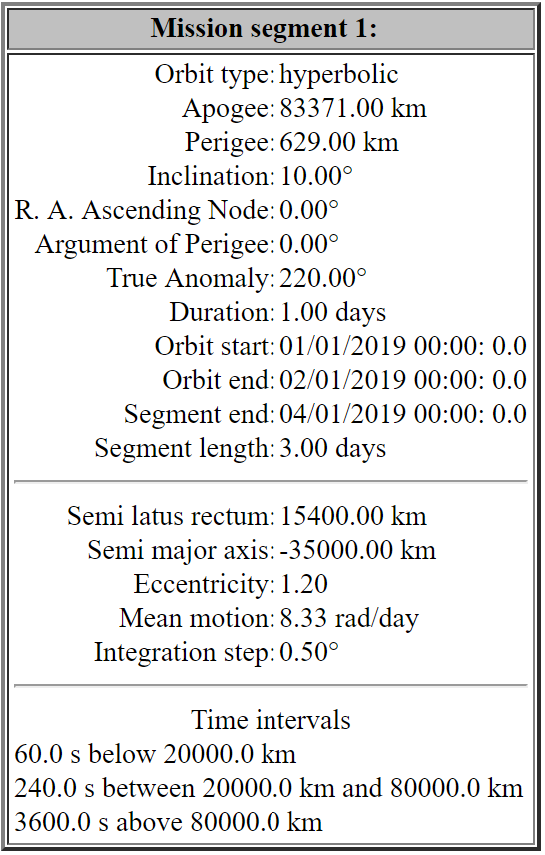
\includegraphics[scale=1]{figures/OrbitParameters.png}
\caption{Parameters of Willzyx I trajectory}
\label{OrbitParam}
\end{figure} 

In figure \ref{OrbitParam} above we can see the parameters of the trajectory followed by Willzyx I. These are the parameters used in order to numerically simulate and plot the orbit. 

\begin{figure}[H]
\centering
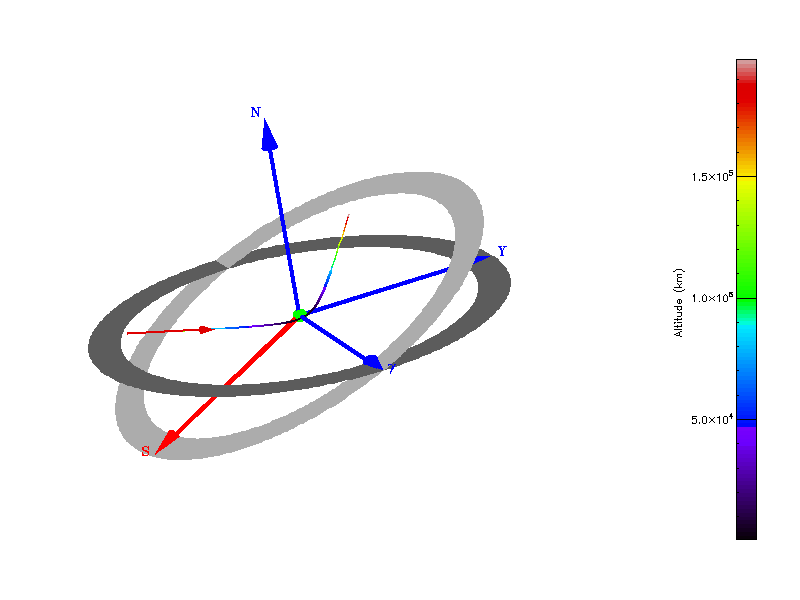
\includegraphics[width=0.68\textwidth]{figures/Trajectory.png}
\caption{Trajectory of the spacecraft during 1 day}
\label{Trajectory}
\end{figure}  

Inf figure \ref{Trajectory} the trajectory of the spacecraft around the Earth is shown. As mentioned before, since this is a hyperbolic trajectory (and therefore not a closed orbit), it will escape Earth after the flyby.

\begin{figure}[H]
\centering
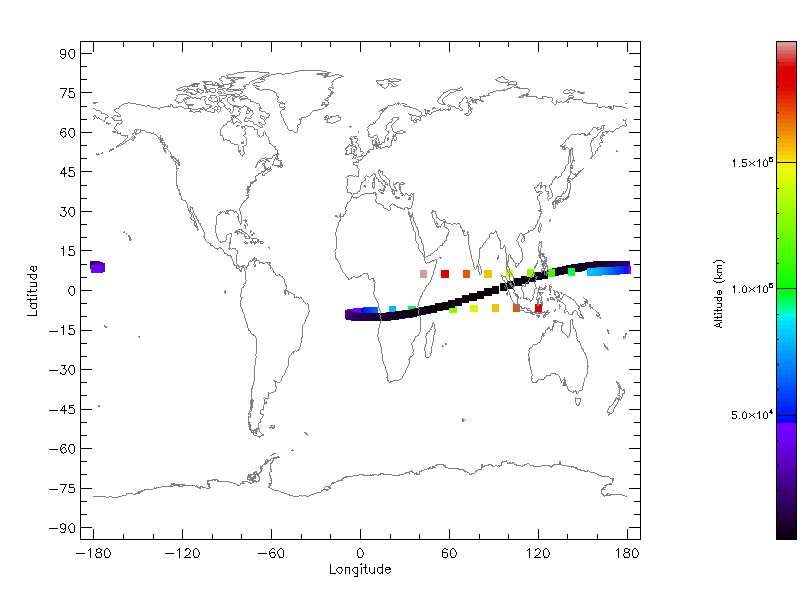
\includegraphics[width=0.78\textwidth]{figures/GroundTrack.png}
\caption{Ground Track of the spacecraft during the flyby}
\label{GroundTrack}
\end{figure}

Figure \ref{GroundTrack} shows the path that Willzyx I will have on the surface of the Earth during the flyby. Due to it's low inclination it will stay very close to the Equator.
